% ============================================================================ %
% Encoding: UTF-8 (žluťoučký kůň úpěl ďábelšké ódy)
% ============================================================================ %

\listofappendices

\priloha{Konfigurační soubory}\label{P_configs}
Konfigurační soubor pro bránu:
\begin{lstlisting}[language=json]
{
  "generic_settings": {
    "verbose": true,
    "log_path": "./log",
    "gateway_id": "gateway1",
    "company": "company"
  },
  "device_settings": {
    "supported_devices": [
      {
        "device_type": 1,
        "device_number": 1
      },
      {
        "device_type": 2,
        "device_number": 1
      }
    ],
    "device_communication_type": "LORA",
    "generator_settings": {
      "device_type": 1,
      "device_number": 1
    },
    "lora_settings": {
      "uart_device_path": "/dev/ttyS0",
      "lora_channel": 2,
      "m0_pin": 4,
      "m1_pin": 5,
      "uart_baudrate": 9600,
      "lora_address": 5156
    }
  },
  "output_settings": {
    "output_type": "MQTT",
    "csv_path": "/home/nothrax/data",
    "mqtt_settings": {
      "hostname": "localhost",
      "port": 1883,
      "username": "test1",
      "password": "test2",
      "ssl": false,
      "ca_file": "",
      "client_cert": "",
      "client_key": ""
    }
  }
}
\end{lstlisting}
Konfigurační soubor pro aplikaci pro nahrávání dat:
\begin{lstlisting}[language=json]
{
  "mqtt_settings": {
    "address": "127.0.0.1",
    "port": 1884,
    "ssl": false,
    "ca_cert": "./ca.pem",
    "cert_file": "./cert.pem",
    "keyfile": "key.pem"
  },
  "timeseries_settings": {
    "address": "127.0.0.1:8042",
    "token": "randomTokenValue"
  },
  "relation_settings": {
    "address": "127.0.0.1",
    "user": "root",
    "password": "example"
  }
}
\end{lstlisting}
Konfigurační soubor pro aplikaci pro získávání dat:
\begin{lstlisting}[language=json]
{
  "flask_settings": {
    "host": "127.0.0.1",
    "port": 5000
  },
  "timeseries_settings": {
    "address": "127.0.0.1:8042",
    "token": "randomTokenValue"
  },
  "relation_settings": {
    "address": "127.0.0.1",
    "user": "root",
    "password": "example"
  }
}
\end{lstlisting}


\priloha{Zapojení měřících zařízení}\label{P_zapojeni}
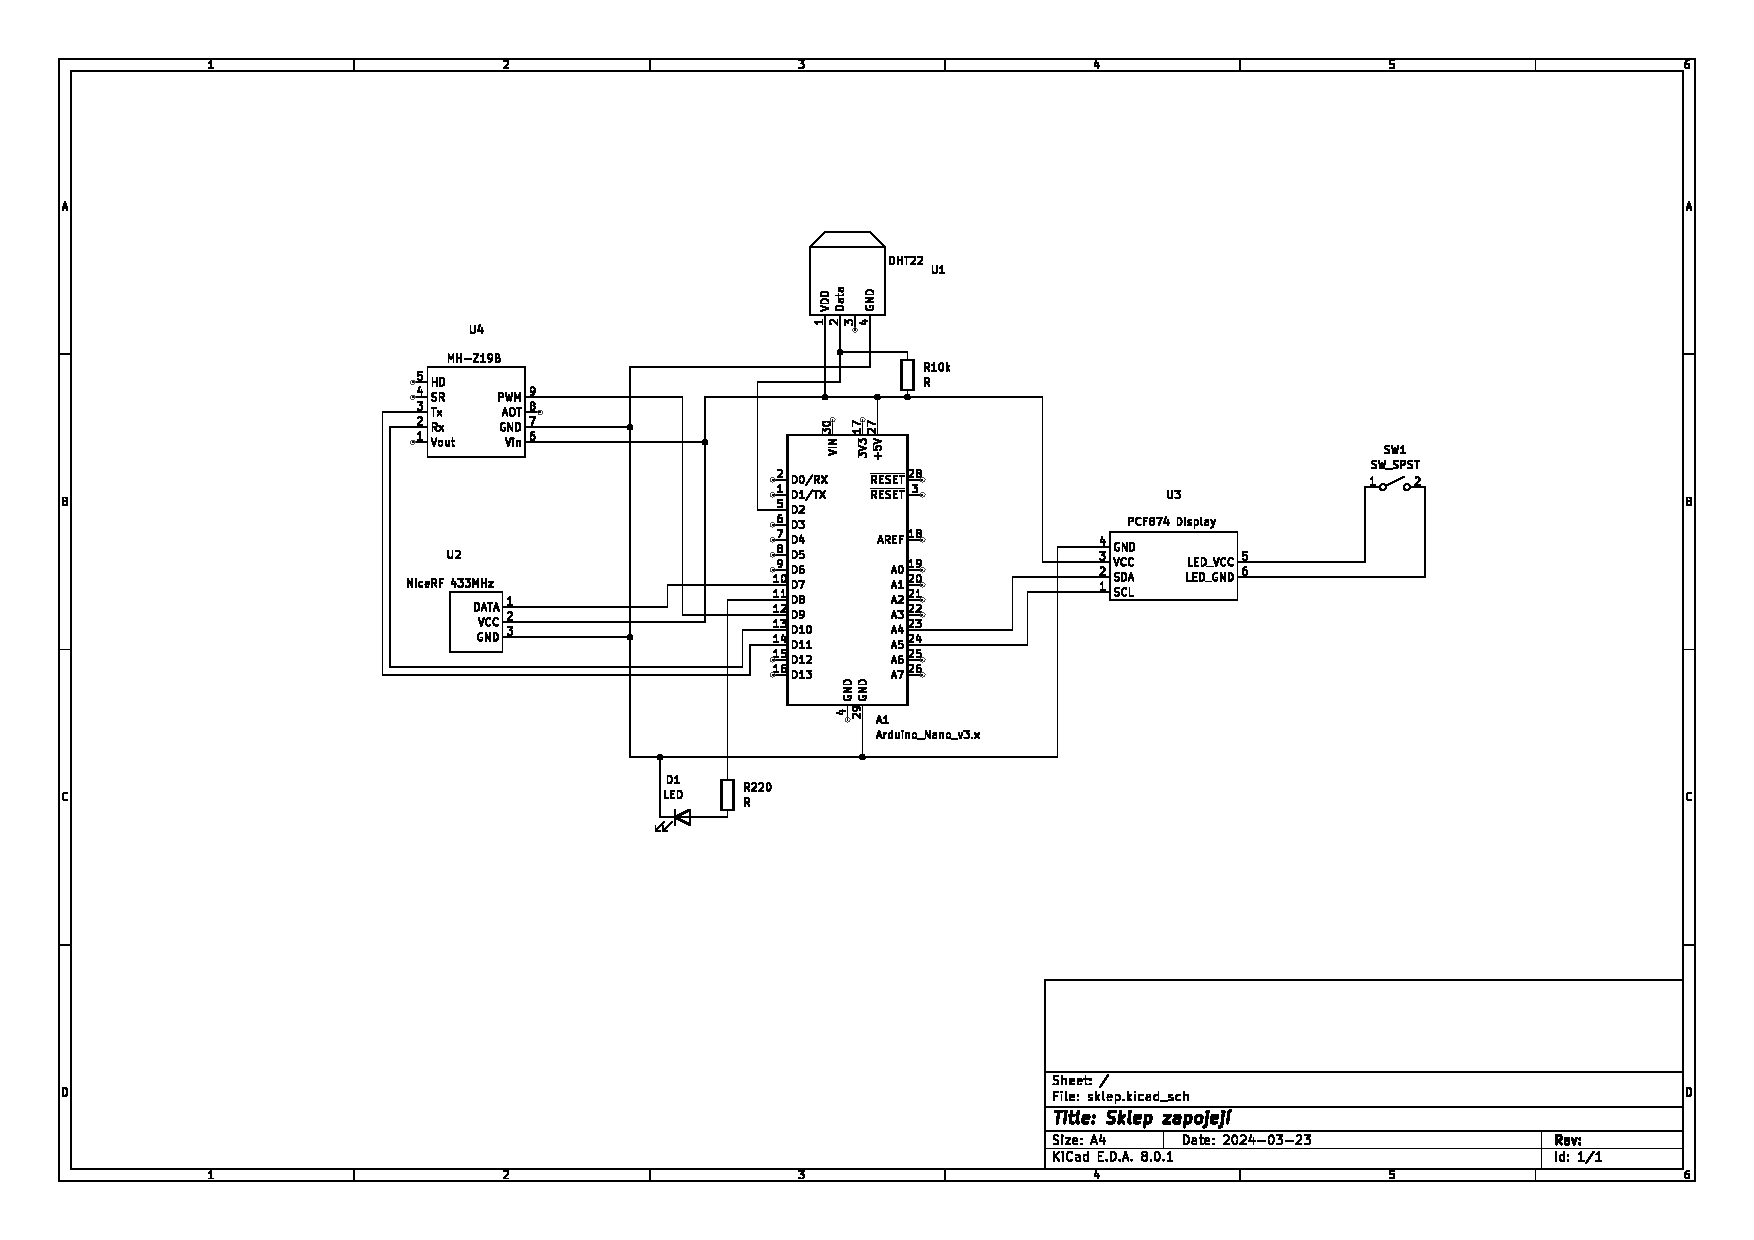
\includepdf[pages=-]{schemata/sklep_zapojeni.pdf}
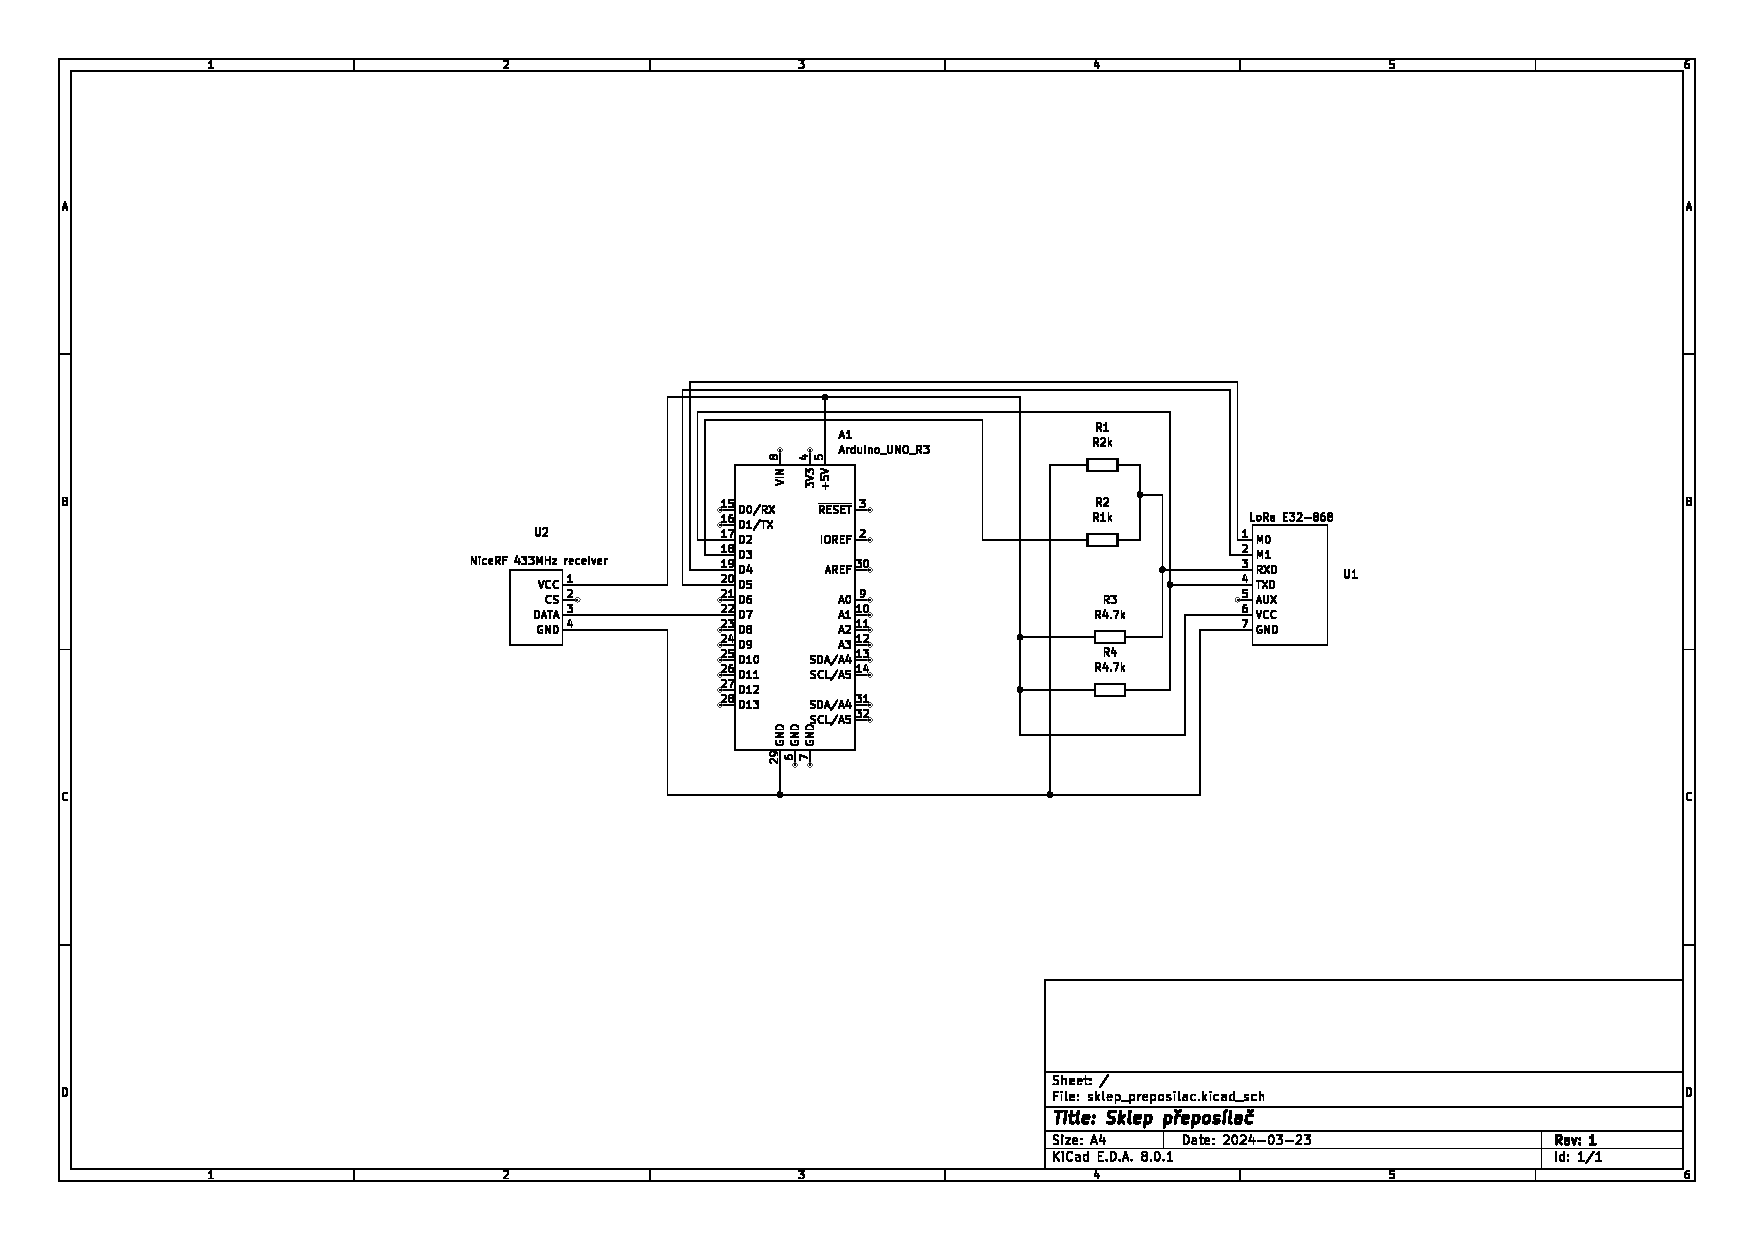
\includepdf[pages=-]{schemata/sklep_preposilac.pdf}
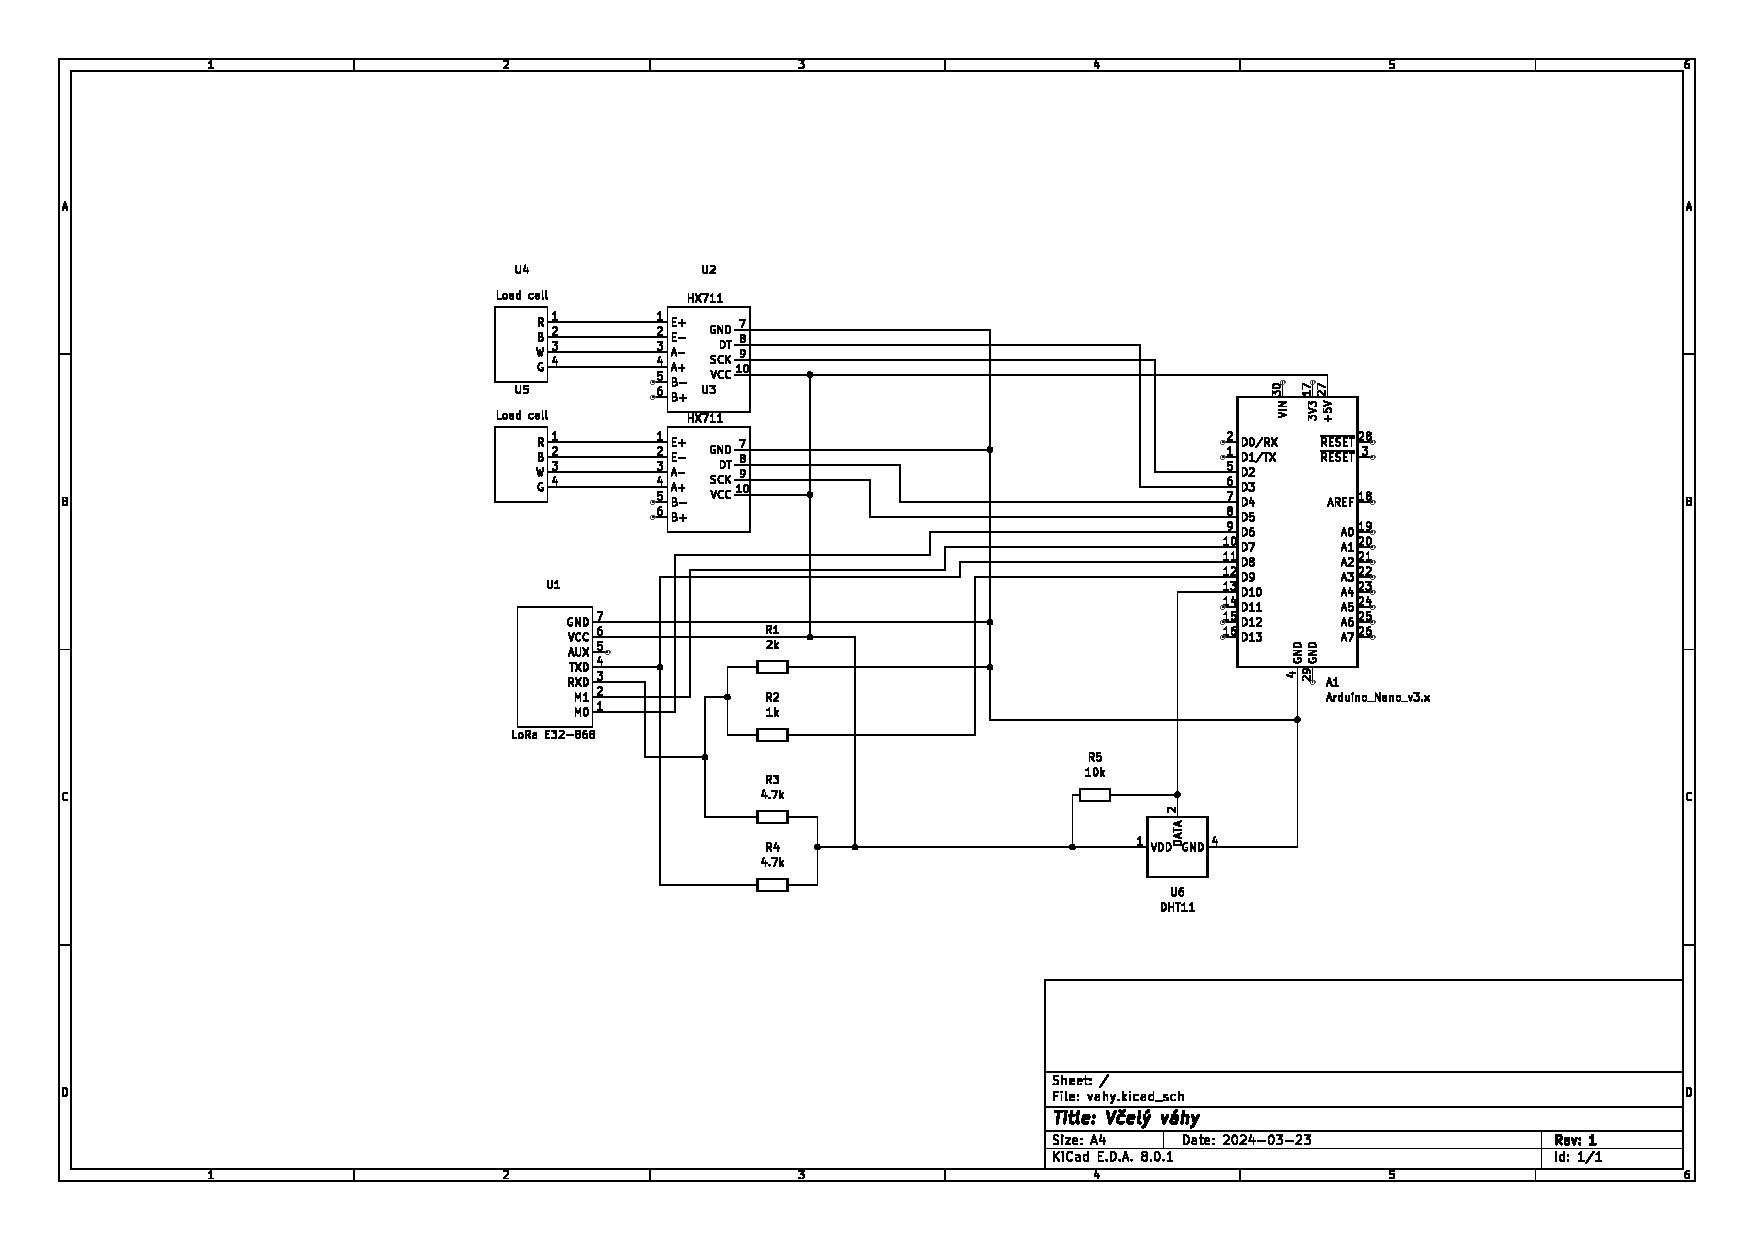
\includepdf[pages=-]{schemata/vahy.pdf}


% ============================================================================ %
